\chapter{La disolución de sólidos iónicos y moleculares}\label{ch:g11:dissolution}

Una pizca de sal removida en agua desaparece en unos segundos; la misma
pizca removida en aceite de cocina se queda en el fondo del vaso, sin
cambiar, todo el tiempo que uno quiera mirarla. Una sartén grasienta
enjuagada bajo el grifo sigue grasienta; una gota de lavavajillas, y la
grasa se despega. ¿Qué decide si una sustancia se \omterm{def:g2:mixing-and-dissolving:dissolve}{disuelve} en un
líquido? La respuesta está en las \omterm{def:g11:polarity-and-cohesion:polar-bond}{cargas parciales} y en las fuerzas
entre partículas del capítulo anterior.

\begin{recall}
La \omterm{def:g6:solutions-and-solubility:solubility}{solubilidad}; los líquidos \omterm{def:g6:solutions-and-solubility:miscible}{miscibles} e \omterm{def:g6:solutions-and-solubility:miscible}{inmiscibles}
(\cref{ch:g6:solutions-and-solubility}). Un \omterm{def:g9:ions:ionic-compound}{compuesto iónico} está
formado por \omterm{def:g9:ions:ion}{cationes} y \omterm{def:g9:ions:ion}{aniones} en proporciones que lo hacen neutro
(\cref{ch:g9:ions}). Las \omterm{def:g11:polarity-and-cohesion:polar-molecule}{moléculas polares} y apolares, los \omterm{def:g11:polarity-and-cohesion:hydrogen-bond}{enlaces de
hidrógeno}, las \omterm{def:g11:polarity-and-cohesion:van-der-waals}{interacciones de van der Waals}
(\cref{ch:g11:polarity-and-cohesion}). La \omterm{def:g10:chemical-species:extraction}{extracción líquido--líquido}
(\cref{ch:g10:chemical-species}). La \omterm{def:g10:concentration-and-dilution:molar-concentration}{concentración molar}
(\cref{ch:g10:concentration-and-dilution}).
\end{recall}

\section{La disolución de un sólido iónico}

En un cristal de cloruro de sodio, cada \omterm{def:g9:ions:ion}{ion} sodio \ce{Na+} está rodeado
de \omterm{def:g9:ions:ion}{iones} cloruro \ce{Cl-}, y cada \omterm{def:g9:ions:ion}{ion} cloruro de \omterm{def:g9:ions:ion}{iones} sodio, todos
unidos por la atracción entre cargas opuestas. Las \omterm{def:g7:atoms-and-molecules:molecule}{moléculas} de agua,
polares, son atraídas por esas cargas: su lado del oxígeno ($\delta^-$)
se orienta hacia los \omterm{def:g9:ions:ion}{cationes}, y su lado de los hidrógenos ($\delta^+$),
hacia los \omterm{def:g9:ions:ion}{aniones}.

\begin{definition}[Disociación]\label{def:g11:dissolution:dissociation}
La \emph{disociación}\index{disociacion@disociación} de un sólido iónico en un
\omterm{def:g6:solutions-and-solubility:solute}{disolvente} es la separación de sus \omterm{def:g9:ions:ion}{iones} unos de otros: salen del
cristal y se alejan en la disolución.
\end{definition}

\begin{definition}[Solvatación, hidratación]\label{def:g11:dissolution:solvation}
La \emph{solvatación}\index{solvatacion@solvatación} de una partícula disuelta es el
hecho de quedar rodeada de \omterm{def:g7:atoms-and-molecules:molecule}{moléculas} de \omterm{def:g6:solutions-and-solubility:solute}{disolvente}, unidas a ella por
atracciones; en el agua se llama
\emph{hidratación}\index{hidratacion@hidratación}. El símbolo (aq) después de una
fórmula significa ``hidratado''.
\end{definition}

\begin{proposition}[Las tres etapas de la disolución]\label{prop:g11:dissolution:stages}
Un sólido iónico se \omterm{def:g2:mixing-and-dissolving:dissolve}{disuelve} en agua en tres etapas que ocurren a la
vez: los \omterm{def:g9:ions:ion}{iones} se arrancan del cristal (\omterm{def:g11:dissolution:dissociation}{disociación}), se rodean de
\omterm{def:g7:atoms-and-molecules:molecule}{moléculas} de agua (\omterm{def:g11:dissolution:solvation}{hidratación}) y se reparten por toda la disolución
(dispersión). Para el cloruro de sodio,
\[
  \ce{NaCl(s) -> Na+(aq) + Cl-(aq)} .
\]
\end{proposition}

\begin{proof}
Se admite: las atracciones entre los \omterm{def:g9:ions:ion}{iones} y las \omterm{def:g11:polarity-and-cohesion:polar-molecule}{moléculas polares} de
agua, sumadas, son lo bastante fuertes para sustituir a las que hay
entre los \omterm{def:g9:ions:ion}{iones} del cristal.
\end{proof}

\begin{omfigure}
\begin{tikzpicture}[font=\small]
  % the crystal edge: alternating ions
  \foreach \i in {0,1,2,3,4} \foreach \j in {0,1,2,3} {
    \pgfmathtruncatemacro\k{mod(\i+\j,2)}
    \ifnum\k=0
      \node[om atom, ball color=green!60!black, minimum size=6.4mm] at (0.8*\i,0.8*\j) {};
    \else
      \node[om atom, ball color=violet!70, minimum size=4.0mm] at (0.8*\i,0.8*\j) {};
    \fi
  }
  % a hydrated Na+ that has left: O towards the ion
  \begin{scope}[shift={(5.6,1.8)}]
    \node[om atom, ball color=violet!70, minimum size=4.0mm] (na) at (0,0) {};
    \node[font=\footnotesize] at (0,0) {};
    \foreach \a in {0,90,180,270} {
      \node[aO, minimum size=4.6mm] (o\a) at (\a:0.62) {};
      \node[aH, minimum size=3.2mm] (ha\a) at ($(\a:0.62)+(\a+52:0.42)$) {};
      \node[aH, minimum size=3.2mm] (hb\a) at ($(\a:0.62)+(\a-52:0.42)$) {};
      \begin{scope}[on background layer]
        \draw[bond, line width=1.2pt] (o\a.center) -- (ha\a.center);
        \draw[bond, line width=1.2pt] (o\a.center) -- (hb\a.center);
      \end{scope}
    }
    \node[anchor=north] at (0,-1.35) {\ce{Na+(aq)}};
  \end{scope}
  % a hydrated Cl- that has left: H towards the ion
  \begin{scope}[shift={(8.6,1.4)}]
    \node[om atom, ball color=green!60!black, minimum size=6.4mm] at (0,0) {};
    \foreach \a in {45,135,225,315} {
      \node[aH, minimum size=3.2mm] (h\a) at (\a:0.62) {};
      \node[aO, minimum size=4.6mm] (o\a) at (\a:1.0) {};
      \node[aH, minimum size=3.2mm] (k\a) at ($(\a:1.0)+(\a+75:0.42)$) {};
      \begin{scope}[on background layer]
        \draw[bond, line width=1.2pt] (o\a.center) -- (h\a.center);
        \draw[bond, line width=1.2pt] (o\a.center) -- (k\a.center);
      \end{scope}
    }
    \node[anchor=north] at (0,-1.45) {\ce{Cl-(aq)}};
  \end{scope}
  \node[anchor=north, align=center] at (1.6,-0.45) {el cristal\\
    (\ce{Na+} pequeño, \ce{Cl-} grande)};
\end{tikzpicture}

{\small El cloruro de sodio se \omterm{def:g2:mixing-and-dissolving:dissolve}{disuelve}. Un \omterm{def:g9:ions:ion}{ion} sodio y un \omterm{def:g9:ions:ion}{ion} cloruro
han salido del cristal; cada uno está hidratado. Alrededor del \omterm{def:g9:ions:ion}{catión},
las \omterm{def:g7:atoms-and-molecules:molecule}{moléculas} de agua orientan hacia dentro sus \omterm{def:g7:atoms-and-molecules:atom}{átomos} de oxígeno
(rojos, $\delta^-$); alrededor del \omterm{def:g9:ions:ion}{anión}, sus \omterm{def:g7:atoms-and-molecules:atom}{átomos} de hidrógeno
(blancos, $\delta^+$).}
\end{omfigure}

\section{Las concentraciones de los iones}

\begin{method}[Concentración de cada ion]\label{met:g11:dissolution:ions}
\begin{enumerate}
  \item Escribir la ecuación de disolución, ajustada en \omterm{def:g7:atoms-and-molecules:atom}{átomos} y en
        carga: para el cloruro de calcio,
        \ce{CaCl2(s) -> Ca^{2+}(aq) + 2Cl-(aq)}.
  \item Calcular la cantidad $n$ de sólido disuelto y la concentración
        $c = n / V$ de la disolución en \omterm{def:g6:solutions-and-solubility:solute}{soluto}.
  \item Cada \omterm{def:g9:ions:ion}{ion} tiene la concentración $c$ multiplicada por su
        coeficiente en la ecuación: aquí $[\ce{Ca^{2+}}] = c$ y
        $[\ce{Cl-}] = 2c$.
\end{enumerate}
Los corchetes $[\ldots]$ indican la \omterm{def:g10:concentration-and-dilution:molar-concentration}{concentración molar} de una especie
disuelta.
\end{method}

\begin{example}[El cloruro de calcio]\label{ex:g11:dissolution:cacl2}
% ledger: aw:Ca, aw:Cl
Se \omterm{def:g2:mixing-and-dissolving:dissolve}{disuelven} \qty{5.55}{g} de cloruro de calcio
($M = \qty{111.1}{g/mol}$) para obtener \qty{500.0}{mL} de disolución:
$n = \qty{0.0500}{mol}$, $c = \qty{0.100}{mol/L}$, así que
$[\ce{Ca^{2+}}] = \qty{0.100}{mol/L}$ y
$[\ce{Cl-}] = \qty{0.200}{mol/L}$. La disolución es neutra: $2 \times
0.100$ de carga positiva por litro frente a $1 \times 0.200$ de carga
negativa.
\end{example}

\section{Polaridad y solubilidad}

\begin{proposition}[Lo semejante disuelve a lo semejante]\label{prop:g11:dissolution:like}
Un \omterm{def:g6:solutions-and-solubility:solute}{disolvente} polar, como el agua, \omterm{def:g2:mixing-and-dissolving:dissolve}{disuelve} los sólidos iónicos y las
especies polares, sobre todo las que pueden formar \omterm{def:g11:polarity-and-cohesion:hydrogen-bond}{enlaces de hidrógeno}
con él; un \omterm{def:g6:solutions-and-solubility:solute}{disolvente} apolar, como el ciclohexano o un aceite vegetal,
\omterm{def:g2:mixing-and-dissolving:dissolve}{disuelve} las especies apolares. Los sólidos iónicos se \omterm{def:g2:mixing-and-dissolving:dissolve}{disuelven} muy poco
en los \omterm{def:g6:solutions-and-solubility:solute}{disolventes} apolares, y las especies apolares, muy poco en el
agua.
\end{proposition}

\begin{proof}
Se admite: un \omterm{def:g6:solutions-and-solubility:solute}{soluto} se \omterm{def:g2:mixing-and-dissolving:dissolve}{disuelve} bien cuando las atracciones que puede
formar con el \omterm{def:g6:solutions-and-solubility:solute}{disolvente} son al menos tan fuertes como las que rompe,
entre sus propias partículas y entre las \omterm{def:g7:atoms-and-molecules:molecule}{moléculas} del \omterm{def:g6:solutions-and-solubility:solute}{disolvente}.
\end{proof}

\begin{example}[Tres casos]\label{ex:g11:dissolution:cases}
% ledger: sol:I2-water, sol:I2-heptane
El etanol se \omterm{def:g6:pure-substances-and-mixtures:mixture}{mezcla} con el agua en todas las proporciones: su grupo
\ce{O-H} forma \omterm{def:g11:polarity-and-cohesion:hydrogen-bond}{enlaces de hidrógeno} con el agua. La sal se \omterm{def:g2:mixing-and-dissolving:dissolve}{disuelve} en
agua pero no en aceite. El yodo, \ce{I2}, una \omterm{def:g11:polarity-and-cohesion:polar-molecule}{molécula apolar}, se
\omterm{def:g2:mixing-and-dissolving:dissolve}{disuelve} mal en agua (unos \qty{0.3}{g/L}, una disolución parda), pero
bien en los \omterm{def:g6:solutions-and-solubility:solute}{disolventes} apolares (\qty{17}{g} por kilogramo de heptano,
una disolución violeta).
\end{example}

\section{La extracción líquido--líquido, explicada}

Una \omterm{def:g10:chemical-species:extraction}{extracción líquido--líquido} hace pasar una especie de un \omterm{def:g6:solutions-and-solubility:solute}{disolvente}
a otro, \omterm{def:g6:solutions-and-solubility:miscible}{inmiscible} con el primero, en el que es más soluble. La regla
``lo semejante \omterm{def:g2:mixing-and-dissolving:dissolve}{disuelve} a lo semejante'' indica qué \omterm{def:g6:solutions-and-solubility:solute}{disolvente} elegir.

\begin{inthelab}[Extraer el yodo]
Se vierten \qty{20}{mL} de una \omterm{def:g6:solutions-and-solubility:solute}{disolución acuosa} parda de yodo en un
embudo de \omterm{def:g3:separating-mixtures:decant}{decantación} con \qty{10}{mL} de ciclohexano. Se tapa el
embudo, se agita, se libera la presión por la llave y se deja reposar.
Se forman dos capas: el ciclohexano, menos denso, arriba. La capa
superior es ahora violeta, y la inferior, casi incolora: el yodo ha
pasado al ciclohexano. La capa inferior se vacía por la llave, y el
yodo se recupera en el ciclohexano.
\end{inthelab}

\begin{omfigure}
\begin{tikzpicture}[font=\small, scale=1.15]
  \pic[transform shape] at (0,0) {sepfunnel={orange!55!brown!70}{white}};
  \node[anchor=north, align=center] at (0,-0.15) {antes de agitar};
  \draw[omProp, <-] (0.55,2.1) -- (1.4,2.5) node[right, text=black] {ciclohexano};
  \draw[omProp, <-] (0.45,1.35) -- (1.4,1.2) node[right, text=black,
    align=left] {yodo acuoso\\ (pardo)};
  \pic[transform shape] at (4.6,0) {sepfunnel={orange!10}{violet!60}};
  \node[anchor=north, align=center] at (4.6,-0.15) {después de agitar\\ y dejar reposar};
  \draw[omProp, <-] (5.15,2.1) -- (6.0,2.5) node[right, text=black,
    align=left] {yodo en\\ ciclohexano (violeta)};
  \draw[omProp, <-] (5.05,1.35) -- (6.0,1.2) node[right, text=black,
    align=left] {agua, casi\\ incolora};
\end{tikzpicture}

{\small \omterm{def:g10:chemical-species:extraction}{Extracción} del yodo del agua con ciclohexano. El yodo, apolar,
pasa al \omterm{def:g6:solutions-and-solubility:solute}{disolvente} apolar; el ciclohexano, menos denso que el agua,
flota encima.}
\end{omfigure}

\begin{safety}{\ghs[0.82cm]{GHS02}\ghs[0.82cm]{GHS07}\ghs[0.82cm]{GHS08}\ghs[0.82cm]{GHS09}}
% ledger: ghs:I2, ghs:cyclohexane
El ciclohexano es muy inflamable, sus vapores provocan somnolencia, es
nocivo para los pulmones en caso de ingestión y muy tóxico para los
organismos acuáticos. El yodo es nocivo en contacto con la piel y por
inhalación. Campana extractora, gafas y guantes, ninguna llama cerca; los
residuos orgánicos se recogen.
\end{safety}


\section{Los jabones y las moléculas anfífilas}

\begin{definition}[Hidrófilo, hidrófobo]\label{def:g11:dissolution:hydrophilic}
Una especie o una parte de una \omterm{def:g7:atoms-and-molecules:molecule}{molécula} es
\emph{hidrófila}\index{hidrofila@hidrófila} si es atraída por el agua (grupos
iónicos o polares, grupos que forman \omterm{def:g11:polarity-and-cohesion:hydrogen-bond}{enlaces de hidrógeno}); es
\emph{hidrófoba}\index{hidrofoba@hidrófoba} si no lo es (largas cadenas de \omterm{def:g7:atoms-and-molecules:atom}{átomos}
de carbono e hidrógeno, apolares). Las especies hidrófobas se \omterm{def:g2:mixing-and-dissolving:dissolve}{disuelven}
en las grasas y los aceites.
\end{definition}

\begin{definition}[Molécula anfífila, micela]\label{def:g11:dissolution:amphiphilic}
Una \omterm{def:g7:atoms-and-molecules:molecule}{molécula} o un \omterm{def:g9:ions:ion}{ion} \emph{anfífilo}\index{anfifilo@anfífilo} tiene una cabeza
\omterm{def:g11:dissolution:hydrophilic}{hidrófila} y una cola \omterm{def:g11:dissolution:hydrophilic}{hidrófoba}. En el agua, los \omterm{def:g9:ions:ion}{iones} anfífilos se
agrupan en \emph{micelas}\index{micela}: esferas diminutas con las
colas dentro, fuera del agua, y las cabezas en la superficie, en
contacto con ella.
\end{definition}

\begin{example}[Un jabón]\label{ex:g11:dissolution:soap}
% ledger: aw:C, aw:H, aw:O, aw:Na
El estearato de sodio, \ce{C17H35COONa} ($M = \qty{306.0}{g/mol}$), es
un jabón típico, fabricado a partir de grasas animales o vegetales. En
el agua se \omterm{def:g2:mixing-and-dissolving:dissolve}{disuelve} en forma de \omterm{def:g9:ions:ion}{iones} sodio \ce{Na+} e \omterm{def:g9:ions:ion}{iones} estearato
\ce{C17H35COO-}: una cabeza \ce{-COO-}, iónica, \omterm{def:g11:dissolution:hydrophilic}{hidrófila}, y una cola de
17 \omterm{def:g7:atoms-and-molecules:atom}{átomos} de carbono, \omterm{def:g11:dissolution:hydrophilic}{hidrófoba}.
\end{example}

\begin{omfigure}
\begin{tikzpicture}[font=\small]
  % the stearate ion as a zigzag of 17 carbons + COO-
  \foreach \k in {0,1,2,3,4,5,6,7,8,9,10,11,12,13,14,15,16} {
    \pgfmathsetmacro\y{mod(\k,2)==0 ? 0 : 0.3}
    \coordinate (c\k) at (0.42*\k,\y);
  }
  \draw[line width=0.9pt] (c0) \foreach \k in {1,2,3,4,5,6,7,8,9,10,11,12,13,14,15,16} { -- (c\k) };
  \coordinate (cc) at ($(c16)+(30:0.42)$);
  \begin{scope}[on background layer]
    \fill[omDef!15, rounded corners] ($(cc)+(-0.25,-0.55)$) rectangle ($(cc)+(1.05,0.9)$);
  \end{scope}
  \draw[line width=0.9pt] (c16) -- (cc);
  \draw[line width=0.9pt] (cc) -- ++(90:0.4) node[above] {O};
  \draw[line width=0.9pt] ([xshift=1.5pt]cc) -- ++(90:0.36);
  \draw[line width=0.9pt] (cc) -- ++(-30:0.42) node[right] {O$^-$};
  \draw[omProp] ($(c0)+(0,-0.15)$) -- ++(0,-0.15) -- ($(c16)+(0,-0.3)$) -- ++(0,0.15);
  \node[omProp, anchor=north] at ($(c8)+(0,-0.32)$) {cola hidrófoba (17 átomos de carbono)};
  \node[omDef, anchor=south] at ($(cc)+(0.35,0.9)$) {cabeza hidrófila};
  % the sketch
  \begin{scope}[yshift=-1.9cm]
    \draw[omProp, line width=1.6pt, decorate, decoration={snake, amplitude=1.5pt,
      segment length=6pt}] (2.0,0) -- (5.2,0);
    \fill[omDef] (5.45,0) circle (0.25);
    \node[white, font=\scriptsize\bfseries] at (5.45,0) {$-$};
    \node[anchor=west] at (5.9,0) {el mismo ion, esquematizado};
  \end{scope}
\end{tikzpicture}

{\small El \omterm{def:g9:ions:ion}{ion} estearato. En este dibujo en zigzag, cada vértice de la
cadena es un \omterm{def:g7:atoms-and-molecules:atom}{átomo} de carbono que lleva \omterm{def:g7:atoms-and-molecules:atom}{átomos} de hidrógeno (\ce{CH2}, y
\ce{CH3} en el extremo); un capítulo posterior explica esta notación
abreviada. Debajo, el esquema habitual: una cola ondulada y una cabeza
redonda.}
\end{omfigure}

\begin{proposition}[Cómo quita la grasa el jabón]\label{prop:g11:dissolution:soap}
La grasa es \omterm{def:g11:dissolution:hydrophilic}{hidrófoba} y no se \omterm{def:g2:mixing-and-dissolving:dissolve}{disuelve} en agua. En el agua jabonosa,
las colas de los \omterm{def:g9:ions:ion}{iones} de jabón se \omterm{def:g2:mixing-and-dissolving:dissolve}{disuelven} en la grasa mientras las
cabezas se quedan en el agua; la grasa se rompe en gotitas diminutas,
cada una envuelta en una \omterm{def:g11:dissolution:amphiphilic}{micela} cuya superficie cargada da al agua, y
el agua del aclarado se lleva las gotitas.
\end{proposition}

\begin{proof}
Se admite: se deduce de ``lo semejante \omterm{def:g2:mixing-and-dissolving:dissolve}{disuelve} a lo semejante''
aplicado a cada extremo del \omterm{def:g9:ions:ion}{ion}; las cabezas cargadas del exterior
impiden además que las gotitas vuelvan a unirse, ya que las cargas del
mismo signo se repelen.
\end{proof}

\begin{omfigure}
\begin{tikzpicture}[font=\small]
  \fill[yellow!45!orange!35] (0,0) circle (1.0);
  \node at (0,0) {grasa};
  \foreach \a in {0,20,40,60,80,100,120,140,160,180,200,220,240,260,280,300,320,340} {
    \draw[omProp, line width=1.3pt, decorate, decoration={snake,
      amplitude=1pt, segment length=4pt}] (\a:0.55) -- (\a:1.45);
    \fill[omDef] (\a:1.6) circle (0.15);
  }
  \node[anchor=west, align=left] at (2.4,0.6) {cabezas ($-$) en el agua};
  \node[anchor=west, align=left] at (2.4,-0.4) {colas en la grasa};
  \draw[black!50] (2.4,0.6) -- (1.75,0.45);
  \draw[black!50] (2.4,-0.4) -- (1.05,-0.25);
  \node[font=\small, blue!50!black] at (-2.6,1.4) {agua};
\end{tikzpicture}

{\small Una \omterm{def:g11:dissolution:amphiphilic}{micela} en corte: \omterm{def:g9:ions:ion}{iones} de jabón alrededor de una gotita de
grasa, con las colas hacia dentro y las cabezas cargadas hacia fuera.
Cada \omterm{def:g11:dissolution:amphiphilic}{micela} tiene carga negativa en su superficie, y las \omterm{def:g11:dissolution:amphiphilic}{micelas} se
repelen entre sí.}
\end{omfigure}

\begin{omfigure}
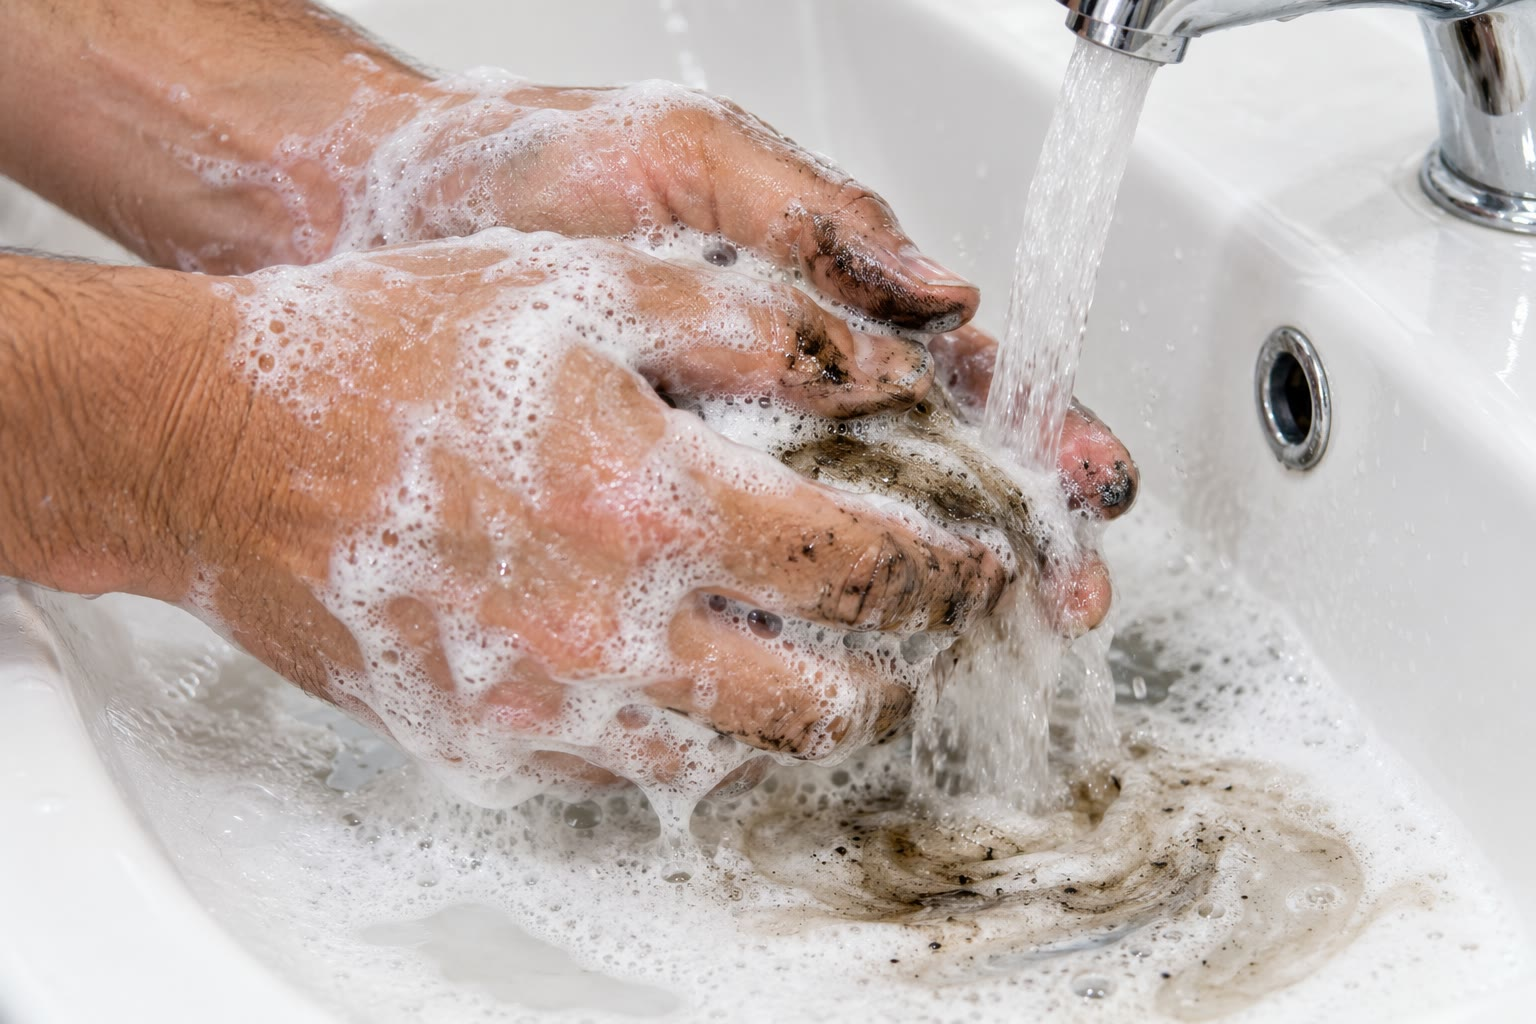
\includegraphics[width=0.48\linewidth]{images/book1/ai/g11-greasy-hands.jpg}

{\small Lavarse unas manos grasientas: el jabón se lleva la grasa en
\omterm{def:g11:dissolution:amphiphilic}{micelas}.}
\end{omfigure}

\begin{remark}[El agua dura y el jabón de cal]\label{rem:g11:dissolution:scum}
El agua dura contiene muchos \omterm{def:g9:ions:ion}{iones} calcio \ce{Ca^{2+}} e \omterm{def:g9:ions:ion}{iones} magnesio
\ce{Mg^{2+}}, disueltos de las rocas por las que ha pasado. Con los
\omterm{def:g9:ions:ion}{iones} estearato forman un \omterm{def:g9:ions:precipitate}{precipitado} (\cref{ch:g9:ions}), el estearato
de calcio:
\[
  \ce{2C17H35COO- + Ca^{2+} -> Ca(C17H35COO)2(s)} .
\]
Este sólido grisáceo es la costra que deja un cerco en el lavabo, y cada
\omterm{def:g9:ions:ion}{ion} de jabón atrapado en ella se pierde para lavar: en agua dura, el
jabón hace poca espuma hasta que se ha añadido lo suficiente para
precipitar todo el calcio.
\end{remark}

\begin{omfigure}
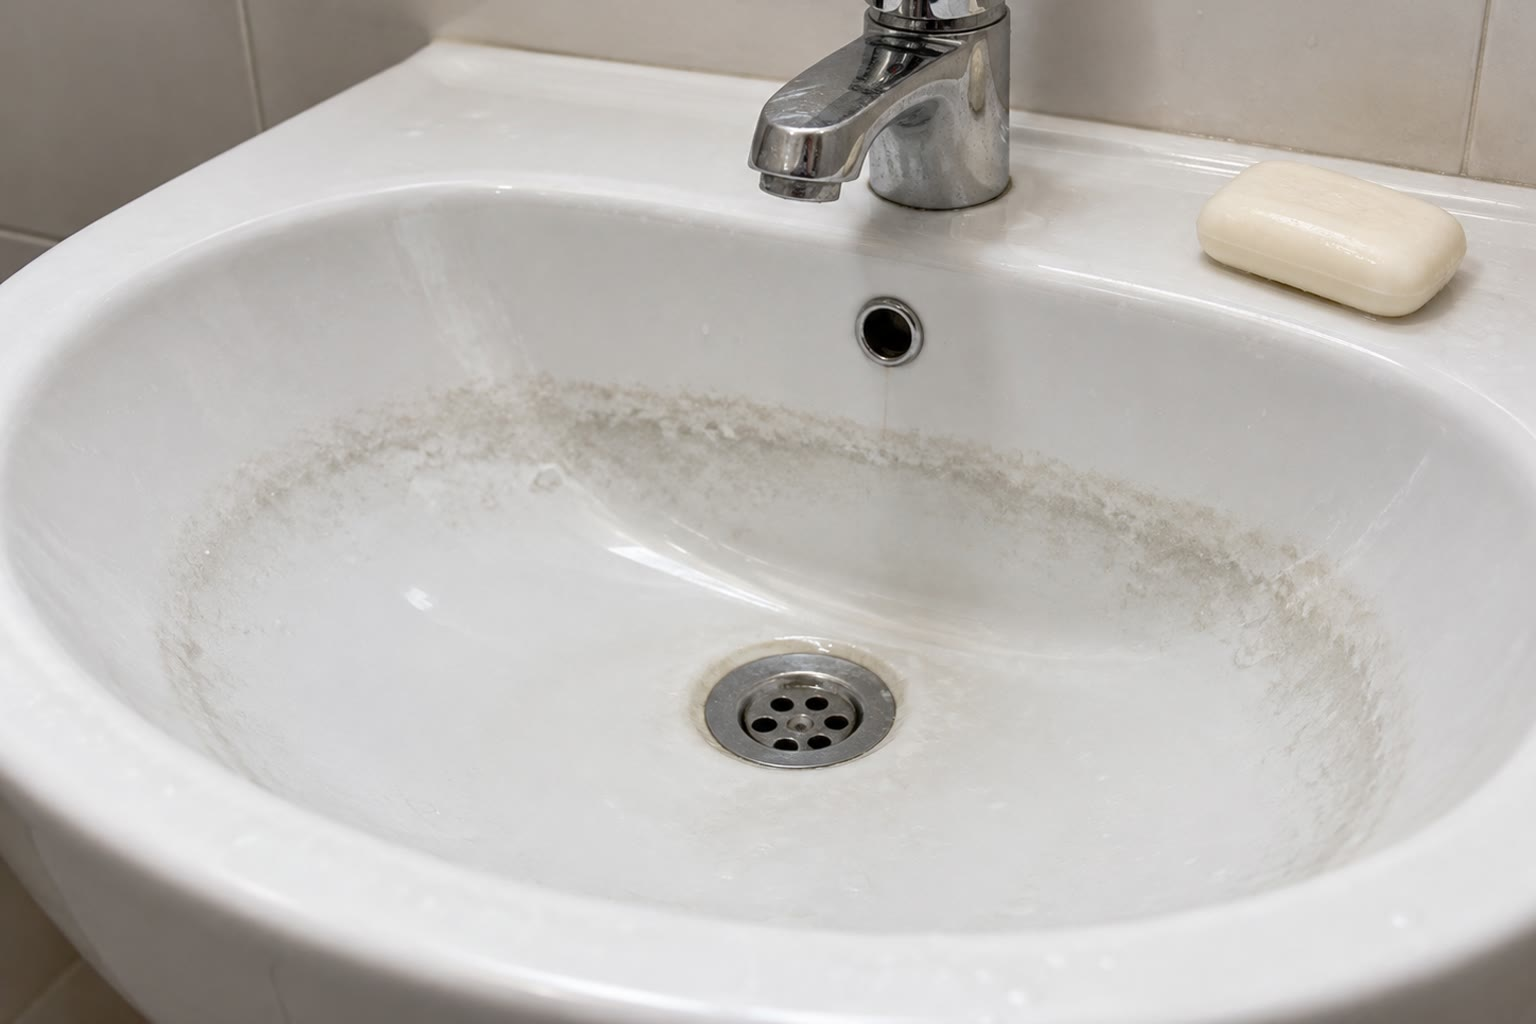
\includegraphics[width=0.45\linewidth]{images/book1/ai/g11-soap-scum.jpg}

{\small Jabón de cal en un lavabo: estearato de calcio, \omterm{def:g9:ions:precipitate}{precipitado} por
el agua dura.}
\end{omfigure}

\section{Ejercicios}


\begin{exercise}[$\star$]\label{exo:g11:dissolution:1}
Escribe las ecuaciones de disolución en agua del cloruro de sodio
\ce{NaCl}, el cloruro de calcio \ce{CaCl2}, el sulfato de sodio
\ce{Na2SO4} y el cloruro de aluminio \ce{AlCl3}.
\end{exercise}

\begin{exercise}[$\star$]\label{exo:g11:dissolution:2}
Una disolución de sulfato de sodio tiene $c = \qty{0.050}{mol/L}$. Da
las concentraciones de los \omterm{def:g9:ions:ion}{iones} sodio y de los \omterm{def:g9:ions:ion}{iones} sulfato.
\end{exercise}

\begin{exercise}[$\star$]\label{exo:g11:dissolution:3}
¿Qué se entiende por \omterm{def:g11:dissolution:solvation}{hidratación} de un \omterm{def:g9:ions:ion}{ion}? ¿Qué extremo de una \omterm{def:g7:atoms-and-molecules:molecule}{molécula}
de agua apunta hacia un \omterm{def:g9:ions:ion}{catión}, y cuál hacia un \omterm{def:g9:ions:ion}{anión}? ¿Por qué?
\end{exercise}

\begin{exercise}[$\star$]\label{exo:g11:dissolution:4}
Se \omterm{def:g2:mixing-and-dissolving:dissolve}{disuelven} \qty{2.67}{g} de cloruro de aluminio para obtener
\qty{200.0}{mL} de disolución. Calcula la concentración de la
disolución y la de cada \omterm{def:g9:ions:ion}{ion}.
\end{exercise}

\begin{exercise}[$\star$]\label{exo:g11:dissolution:5}
Indica qué partes del \omterm{def:g9:ions:ion}{ion} estearato son \omterm{def:g11:dissolution:hydrophilic}{hidrófilas} y cuáles \omterm{def:g11:dissolution:hydrophilic}{hidrófobas},
y di por qué.
\end{exercise}

\begin{exercise}[$\star\star$]\label{exo:g11:dissolution:6}
¿Qué \omterm{def:g6:solutions-and-solubility:solute}{disolvente}, el agua o el ciclohexano, elegirías para \omterm{def:g2:mixing-and-dissolving:dissolve}{disolver}: la
sal; la cera de una vela (largas cadenas hidrocarbonadas); el azúcar
(muchos grupos \ce{O-H}); el yodo? Justifica cada elección.
\end{exercise}

\begin{exercise}[$\star\star$]\label{exo:g11:dissolution:7}
El etanol \ce{CH3-CH2-OH} se \omterm{def:g6:pure-substances-and-mixtures:mixture}{mezcla} con el agua en todas las
proporciones, pero el hexano \ce{C6H14} no se \omterm{def:g6:pure-substances-and-mixtures:mixture}{mezcla} con el agua.
Explícalo.
\end{exercise}

\begin{exercise}[$\star\star$]\label{exo:g11:dissolution:8}
Mira la figura de la \omterm{def:g11:dissolution:amphiphilic}{micela}. ¿Por qué las colas están dentro y las
cabezas fuera? ¿Por qué dos \omterm{def:g11:dissolution:amphiphilic}{micelas} no se unen en una gota de grasa más
grande?
\end{exercise}

\begin{exercise}[$\star\star$]\label{exo:g11:dissolution:9}
Un aroma vegetal está disuelto en agua. Para extraerlo, un químico
puede usar etanol o ciclohexano. ¿Cuál es adecuado, y por qué no lo es
el otro (piensa en la miscibilidad)?
\end{exercise}

\begin{exercise}[$\star\star$]\label{exo:g11:dissolution:10}
En la \omterm{def:g10:chemical-species:extraction}{extracción} del yodo, ¿por qué la capa de ciclohexano queda arriba?
¿Qué capa se vacía por la llave? ¿Dónde está el yodo al final?
\end{exercise}

\begin{exercise}[$\star\star$]\label{exo:g11:dissolution:11}
Se agita una disolución azul de sulfato de cobre con ciclohexano. ¿Qué
le pasa al color azul? Explícalo.
\end{exercise}

\begin{exercise}[$\star\star\star$]\label{exo:g11:dissolution:12}
¿Qué masa de cloruro de calcio hay que \omterm{def:g2:mixing-and-dissolving:dissolve}{disolver} para obtener
\qty{250.0}{mL} de una disolución en la que
$[\ce{Cl-}] = \qty{0.300}{mol/L}$?
\end{exercise}

\begin{exercise}[$\star\star\star$]\label{exo:g11:dissolution:13}
Se halla que una muestra de agua de mar contiene \qty{0.010}{mol/L} de
\omterm{def:g9:ions:ion}{iones} calcio y \qty{0.053}{mol/L} de \omterm{def:g9:ions:ion}{iones} magnesio. Explica por qué el
jabón corriente hace muy poca espuma en el agua de mar. ¿Cuánto
estearato de sodio precipitarían solo los \omterm{def:g9:ions:ion}{iones} calcio de un litro de
agua de mar?
\end{exercise}

\begin{exercise}[$\star\star\star$]\label{exo:g11:dissolution:14}
Se \omterm{def:g2:mixing-and-dissolving:mix}{mezclan} \qty{100.0}{mL} de disolución de cloruro de sodio de
\qty{0.20}{mol/L} con \qty{100.0}{mL} de disolución de cloruro de calcio
de \qty{0.10}{mol/L}. No se forma ningún \omterm{def:g9:ions:precipitate}{precipitado}. Calcula las
concentraciones de \ce{Na+}, \ce{Ca^{2+}} y \ce{Cl-} en la \omterm{def:g6:pure-substances-and-mixtures:mixture}{mezcla}, y
comprueba que es neutra.
\end{exercise}

\begin{exercise}[$\star\star\star$]\label{exo:g11:dissolution:15}
% ledger: sol:I2-water, sol:I2-heptane, rho:heptane
El yodo se \omterm{def:g2:mixing-and-dissolving:dissolve}{disuelve} a razón de unos \qty{0.3}{g} por litro de agua y
\qty{17}{g} por kilogramo de heptano. El heptano tiene una densidad de
unos \qty{0.68}{kg/L}. ¿Cuántas veces más yodo puede contener un litro
de heptano que un litro de agua? ¿Qué significa esto para una
\omterm{def:g10:chemical-species:extraction}{extracción}?
\end{exercise}

\section{Problema: El jabón y el agua dura}

\begin{problem}[{Problema de fin de semana --- ¿cuánto jabón
desperdicia en forma de costra un baño de agua dura?}]
\label{pb:g11:dissolution:1}
% ledger: aw:Ca, aw:Mg, aw:C, aw:H, aw:O, aw:Na
Un agua del grifo contiene \qty{120}{mg} de \omterm{def:g9:ions:ion}{iones} calcio y \qty{24}{mg}
de \omterm{def:g9:ions:ion}{iones} magnesio por litro. Se llena una bañera con \qty{150}{L}, y la
persona que se baña usa un jabón de estearato de sodio,
\ce{C17H35COONa}.

\medskip
\noindent\textbf{Parte I --- Lo que hay en el agua.}
\begin{enumerate}
  \item ¿De dónde vienen los \omterm{def:g9:ions:ion}{iones} calcio y magnesio del agua del
        grifo?
  \item Calcula las \omterm{def:g10:concentration-and-dilution:molar-concentration}{concentraciones molares} de los \omterm{def:g9:ions:ion}{iones} calcio y de los
        \omterm{def:g9:ions:ion}{iones} magnesio.
  \item Los \omterm{def:g9:ions:ion}{iones} calcio van acompañados de \omterm{def:g9:ions:ion}{iones} hidrogenocarbonato,
        \ce{HCO3-}, como si se hubiera disuelto hidrogenocarbonato de
        calcio \ce{Ca(HCO3)2}. Escribe esa ecuación de disolución y
        deduce la concentración de \omterm{def:g9:ions:ion}{iones} hidrogenocarbonato que acompaña
        al calcio.
  \item ¿Qué cantidad de \omterm{def:g9:ions:ion}{iones} calcio contiene la bañera?
\end{enumerate}

\medskip
\noindent\textbf{Parte II --- El jabón.}
\begin{enumerate}[resume]
  \item Calcula la \omterm{def:g10:the-mole:molar-mass}{masa molar} del estearato de sodio.
  \item Escribe su ecuación de disolución en agua.
  \item ¿Qué parte del \omterm{def:g9:ions:ion}{ion} estearato es \omterm{def:g11:dissolution:hydrophilic}{hidrófila} y cuál \omterm{def:g11:dissolution:hydrophilic}{hidrófoba}?
        ¿Por qué se dice que es \omterm{def:g11:dissolution:amphiphilic}{anfífilo}?
  \item Describe una \omterm{def:g11:dissolution:amphiphilic}{micela} y explica cómo quita la grasa de la piel.
  \item ¿Por qué hay que \omterm{def:g2:mixing-and-dissolving:dissolve}{disolver} el jabón en agua, y no en aceite, para
        lavar?
\end{enumerate}

\medskip
\noindent\textbf{Parte III --- La costra.}
\begin{enumerate}[resume]
  \item Escribe la ecuación de la \omterm{def:g9:ions:precipitate}{precipitación} del estearato de calcio.
        Comprueba que está ajustada en carga.
  \item Rellena la \omterm{def:g10:reaction-progress-table:extent}{tabla de avance} para \qty{1.00}{L} del agua del grifo
        y un exceso de \omterm{def:g9:ions:ion}{iones} estearato. ¿Qué \omterm{def:g7:chemical-reactions:reactant}{reactivo} es el limitante?
  \item ¿Qué cantidad de \omterm{def:g9:ions:ion}{iones} estearato se pierde por litro con el
        calcio?
  \item Calcula la \omterm{def:g10:the-mole:molar-mass}{masa molar} del estearato de calcio y la masa de
        costra formada por litro.
  \item El estearato de magnesio precipita del mismo modo. ¿Qué cantidad
        de estearato se llevan por litro los \omterm{def:g9:ions:ion}{iones} magnesio?
\end{enumerate}

\medskip
\noindent\textbf{Parte IV --- El baño.}
\begin{enumerate}[resume]
  \item ¿Qué cantidad de \omterm{def:g9:ions:ion}{iones} estearato precipita el calcio de toda la
        bañera?
  \item ¿Qué masa de jabón es eso?
  \item Sumando el magnesio, ¿qué masa de jabón se desperdicia en
        total?
  \item Las pastillas de jabón pesan unos \qty{100}{g}. ¿Cuántas
        pastillas se lleva solo el calcio?
  \item Da la respuesta final: ¿qué masa de jabón desperdicia en forma
        de costra el calcio de un baño de \qty{150}{L} de esta agua?
\end{enumerate}
\end{problem}
